\chapter{Implementation}

%The implementation should look at any issues you encountered as you tried to implement your design. During the work, you might have found that elements of your design were unnecessary or overly complex; perhaps third party libraries were available that simplified some of the functions that you intended to implement. If things were easier in some areas, then how did you adapt your project to take account of your findings?

%It is more likely that things were more complex than you first thought. In particular, were there any problems or difficulties that you found during implementation that you had to address? Did such problems simply delay you or were they more significant?

%You can conclude this section by reviewing the end of the implementation stage against the planned requirements.
This chapter discusses the implementation challenges of image processing, handwriting training and the creation of the web application. It will provide details on issues overcome, whilst identifying where issues may still persist.
\section{Image processing} \label{imp:image_proces}
Image processing would prove to be an integral part of the application. Pre-processing of the image would be needed to improve the likelihood of Tesseract correctly identifying the characters. This went through several iterative prototypes prior to outputting a fully binarised image.
\subsection{Optimising Tesseract}
Prior to OpenCV being used as the image processing tool several attempts were made to binarise an image using ImageMagick. In sprint zero, converting the image to grey-scale was attempted but this returned poor results from Tesseract. The next iteration of the script was to convert the image to monochrome, this binarised the image, but left a lot of additional noise. It was then suggested by Dr Hannah Dee to use OpenCV for the binarisation process.

\subsubsection{Otsu}
Otsu \cite{citeulike:2917492} is a binarisation technique which essentially converts an image to black and white. Otsu is a global thresholding algorithm, where it uses the whole image for pixel comparison. This is unlike local thresholding algorithms where comparisons are made on smaller segments of the image \cite{citeulike:6044081}.

Images of notes will often have non-uniform lighting; shadows will often be displayed as a user takes a photo. This is problematic for Otsu as shadows will affect the whole picture for a global thresholding algorithm.

\begin{figure}[H]
  \centering
  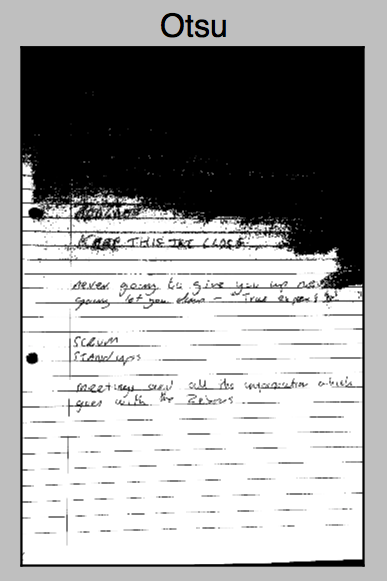
\includegraphics{images/OTSU}
  \caption{The use of Otsu binarisation technique on an image with a little shadow across the image}
  \label{fig:OTSU}
\end{figure}

Figure \ref{fig:OTSU} shows the Otsu binarisation method used on an image with the a slight shadow over the top right of the image. It can be clearly seen that the binarisation segments the image into two distinct regions: the bottom half is white whereas the top half is black. It can be concluded that this would not be a sufficient solution for identifying characters, when specific regions of the image are unreadable.

Otsu attempts to segment the grey-level from the image into a series of histograms. Otsu then determines the optimal threshold value by ``maximising the discriminant measure'' \cite{citeulike:2917492}. Essentially, Otsu attempts to maximise the margin between the histograms, this margin would then act as the threshold value as to whether a pixel is segmented into either a foreground or background pixel \cite{citeulike:14021372}.

Hewlett-Packard, the creator of Tesseract, describe Otsu as its underlying pre-processing algorithm when converting the image prior to extracting textlines and characters \cite{citeulike:13931186}. Once the spike work was completed with Otsu, shown in Figure \ref{fig:OTSU}, it was clear to identify that Tesseract would find it difficult to identify the characters from the image when the output was so poorly binarised.

Overall Otsu, although it is a very reliable binarisation method, suffers from imposed shadows over images.

\subsubsection{Adaptive threshold} \label{section:threshold}
As Tesseract uses Otsu as its pre-processing step, using an image which has been binarisated with Otsu already would not be advantageous in improving the accuracy of the characters detected. As a result, the next iteration evaluates an adaptive threshold technique.

Adaptive threshold calculates the threshold over a series of smaller segments in the image \cite{citeulike:14021401}. As a result shadows have a smaller impact over the whole image, due to adaptive threshold being a local threshold technique. This makes adaptive thresholding rewarding for non-uniform lighting situations, as it becomes more invariant to shadows.

Using the OpenCV library there was two options with adaptive threshold \cite{citeulike:14021409}:
\begin{enumerate}
  \item Gaussian adaptive threshold: the weighted sum of the neighborhood.
  \item Mean adaptive threshold: the mean of the neighborhood.
\end{enumerate}

\begin{figure}[H]
  \centering
  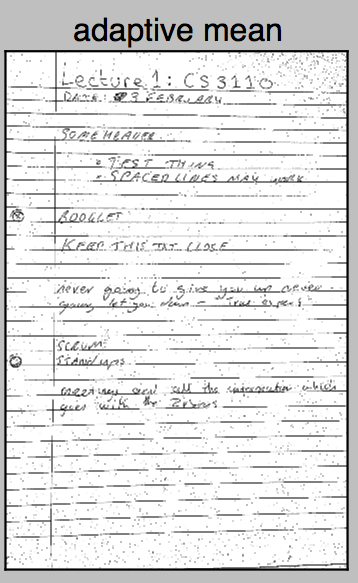
\includegraphics{images/adaptive_mean}
  \caption{Adaptive mean threshold algorithm on a note, showing binarisation but there is still noise in the image.}
  \label{fig:adaptive_mean}
\end{figure}

Mean adaptive threshold uses a specific block size around a given pixel. If the block size was four, then the neighbourhood size would be four and calculations would be made to calculate the mean pixel value in that block. The mean value is selected as the thresholding value for the pixels inside the block; each of the pixels will then be identified as either foreground or background pixels \cite{citeulike:14021401}. Figure \ref{fig:adaptive_mean} shows mean adaptive threshold being used on an image. An additional issue present with the adaptive mean is the noise pixels; there are considerable amounts of noise polluting the image.

Gaussian adaptive threshold differs from the mean adaptive threshold, as instead of calculating the mean value over the block size, it first uses a Gaussian value over blocksize. A Gaussian weight is calculated dynamically depending on the blocksize used for the thresholding. Every pixel inside the block is then multiplied by the Gaussian, and an average value is then taken across the pixels which is used as a threshold. Like the mean adaptive threshold, this is then used to determine if the pixel is foreground or background \cite{bradski2008learning}\cite{citeulike:14021401}.


\begin{figure}[H]
  \centering
  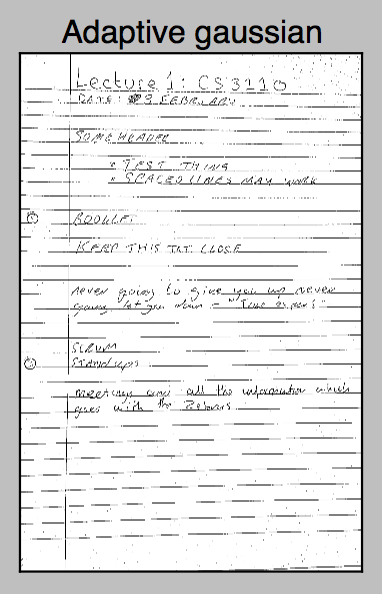
\includegraphics{images/adaptive_gaussian}
  \caption{Adaptive Gaussian used over the image, showing a lot smoother of an image}
  \label{fig:adaptive_gaussian}
\end{figure}

Figure \ref{fig:adaptive_gaussian} shows the adaptive Gaussian being used to binarise an image. The output clearly does not have a shadow overlaying the image and there is less noise pixels than the mean adaptive thresholding.

\begin{figure}[H]
  \centering
  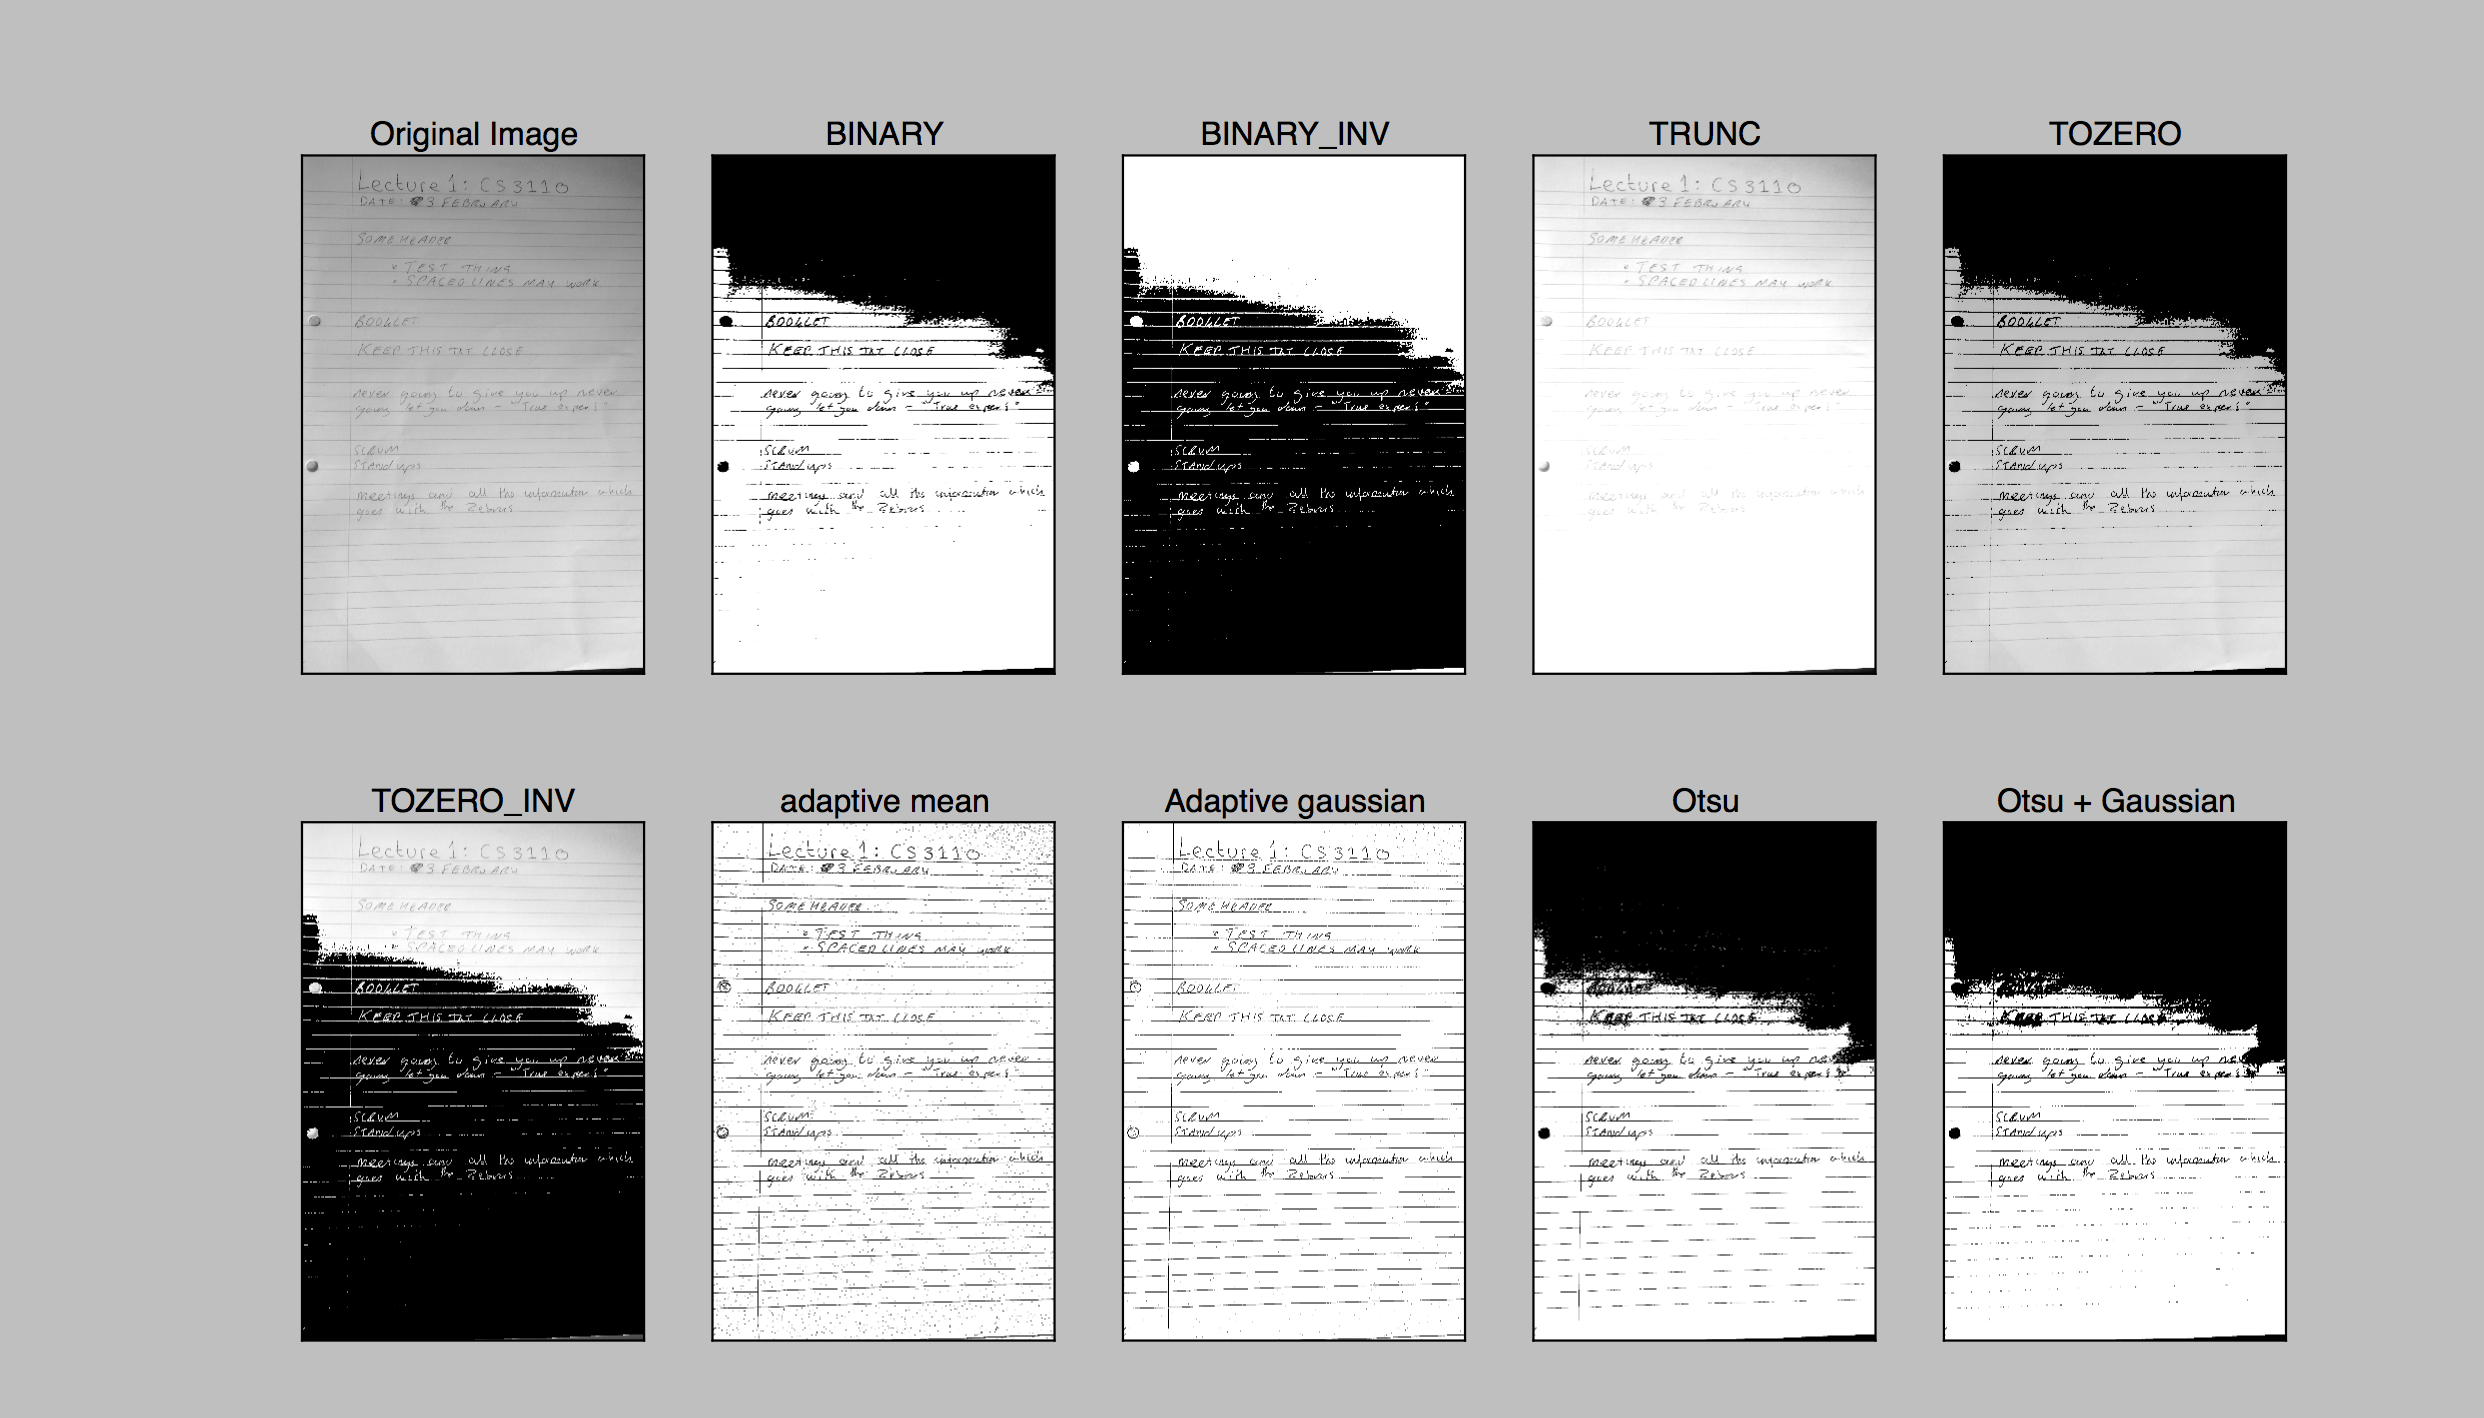
\includegraphics[scale=0.3]{images/thresholding_options}
  \caption{A variety of thresholding techniques used on the same note, showing adaptive threshold resulting in the best output.}
  \label{fig:thresholding_options}
\end{figure}

Figure \ref{fig:thresholding_options} displays additional types of the thresholding that were investigated throughout the iterative process. The Gaussian adaptive threshold provides the clearest results from visual inspection of the different thresholding techniques experimented. As a result, the Gaussian adaptive threshold will be continued to be improved upon throughout a series of iterations to reduce additional noise, via morphological operations to aid in smoothing.

\section{Lined paper}
Initially normal lined paper was used for notes in the project, but after the binarisation process it left too much noise. Further smoothing of the image did not remove the noise, so bespoke lined paper was created to aid in removing the lines but keeping the text uniformly straight. Refer to Appendix \cite{appendix:image_processing}, Section \cite{processing:pre-line}.

\subsection{Filtering the blue lines}
Over a series of iterations, the primary objective was to remove the blue lines from the image. Examples of the lined paper can be found in Appendix \ref{appendix:image_processing}.

\begin{algorithm} [H]
\begin{algorithmic}[1]
  \Function{remove\_lines}{}
    \State image $\gets$ read\_image\_as\_grayscale()
    \State lower\_black $\gets$ np.array([0,0,0])
    \State upper\_black $\gets$ np.array([175,20, 95])
    \State mask\_black $\gets$ cv2.inRange(erode, lower\_black, upper\_black)
    \State mask[np.where(mask\_black == 0)] $\gets$ 255
  \EndFunction
  \end{algorithmic}
  \caption{Initial removing the blue lines algorithm}
  \label{algorithm:threshold1}
\end{algorithm}

Algorithm \ref{algorithm:threshold1} attempted to filter all the colour values between a grey and a black range. By restricting it to a specific range it was intended to bypass the blue lines. However, the blue lines would still contain dark pixels - so only segments of the line would be removed.

\begin{figure}[H]
  \centering
  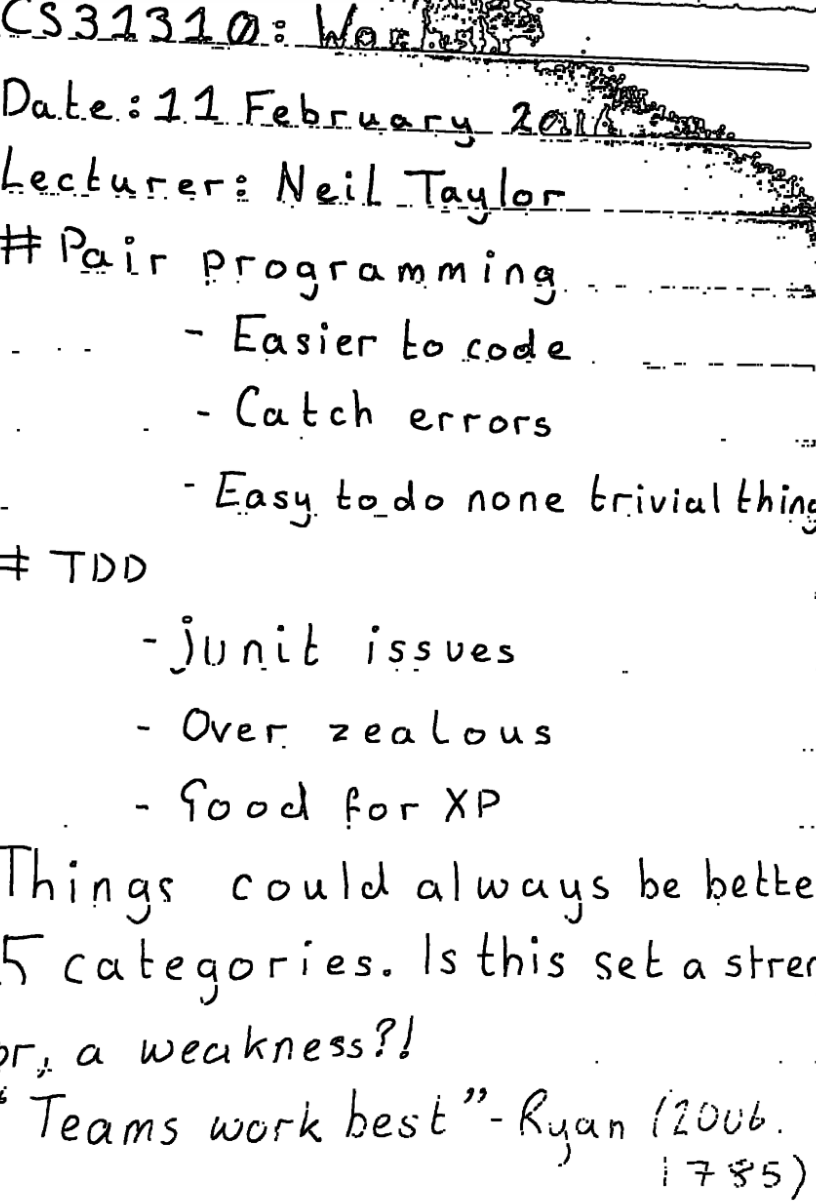
\includegraphics[scale=0.5]{images/removed_lines_still_noise}
  \caption{An example output from the algorithm \ref{algorithm:threshold1}. There is still significant amounts of noise in the image.}
  \label{fig:remove_lines_noise}
\end{figure}

Different morphological operations were used on the image in an attempt to clear the noise pixels. Erosion operations were used, by passing a kernel over the image essentially removing small black noise pixels from the white background whilst expanding the darker pixels, enhancing the text on the page \cite{citeulike:14024957}. Dilation is essentially the opposite: a kernel is passed over the image, and the white background areas get larger and the black text gets thinner; this has the effect of removing the characters quality \cite{citeulike:14024957}.

The result of the morphological operations ended up reducing the quality of the segmentation, as shown in Figure \ref{fig:remove_lines_noise}. This highlighted further iterations were needed for an improved output.

\subsection{Only extracting the text}
There was no simplistic way to identify and filter the lines, therefore it was decided that the text will just be extracted.

OpenCV has an example of line extraction and binarsation \cite{citeulike:14006256}. From the example, structuring elements were used to extract the text from the image. Further erosion and dilation were used to remove additional noise. Throughout the process, masks were used to transfer the state of the image to another mask. An example is transferring the text to a mask, but had an unwanted side effect that line noise way transferred too.

Due to the text having connected pixels, unlike the eroded noise, then connected components were used to identify characters. As a result of  morphological operations the lines were no longer connected. The identified characters were copied to a final mask.

Further smoothing cleared up the image. After a series of iterations the binarisation process was complete.

\begin{figure}[H]
  \centering
  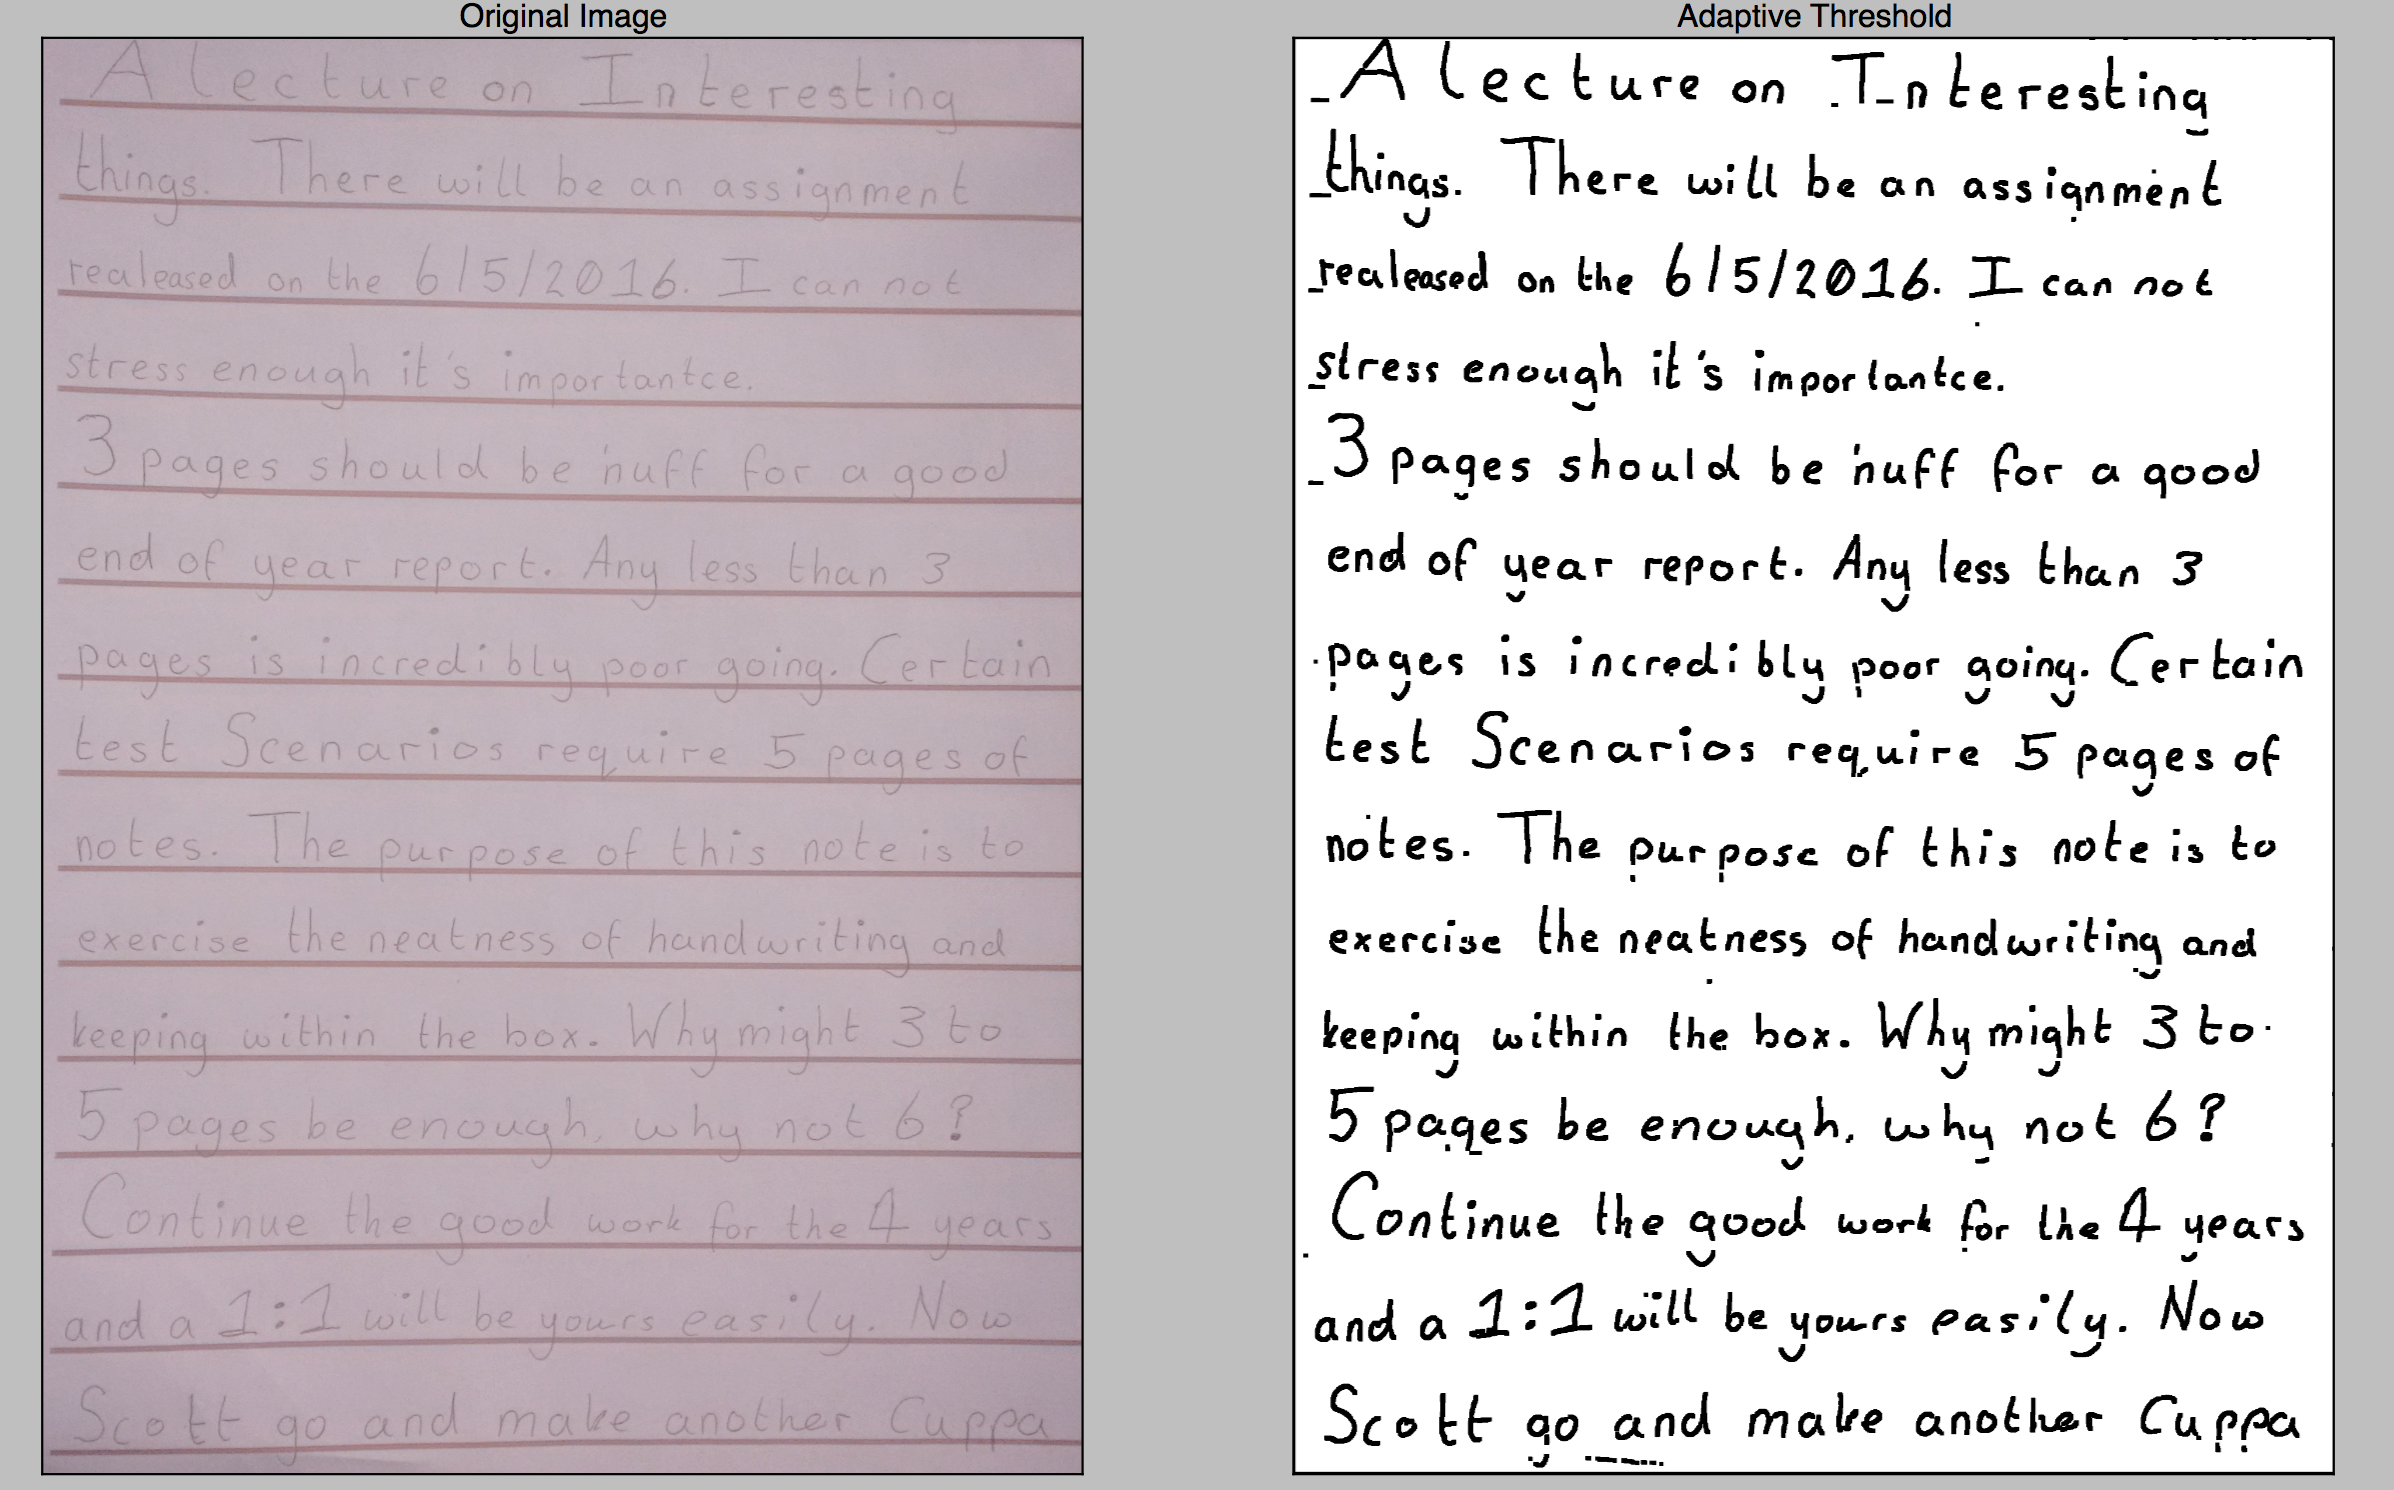
\includegraphics[scale=0.3]{images/hard_image}
  \caption{A poor quality image has been binarised successfully with little noise.}
  \label{fig:poor_quality}
\end{figure}

Figure \ref{fig:poor_quality} shows the result of the binarisation script. Adaptive threshold works well on the image, due to local thresholding not being affected by shadows. Images can be taken in non-uniform lighting and it will produce a fully binarised image. There were issues which affected the implementation such as changing to a bespoke lined paper. Overall the binarisation segmentation works well. Further examples can be found in Appendix \ref{appendix:image_processing}.

\section{Handwriting training}
The training of handwriting was a constant task through out the sprints. It was initially proving cumbersome in the early sprints. After the changes implemented from Section \ref{section:threshold} the results from the handwriting recognition improved considerably.

\subsection{Training process}
Tesseract's training was a methodical process. Tesseract's GitHub wiki \cite{citeulike:13926796} and Gonzalez \cite{citeulike:13920943}, provided great reference tools on how to train the data.

{{\ttfamily \hyphenchar\the\font=`\-}%
Firstly, as handwriting was being trained a new language would have to be created. Each training example has a specific format which must be adhered to: \texttt{lang.font.expNumber.tiff}. The file is then run through the Tesseract training process using \texttt{batch.nochop makebox} command, on the specific language \texttt{eng.ryan.exp2a}; this created  a box file for the given training example. The box file contains the characters which Tesseract believes are in the image; each line is a new character as shown below:
\begin{center}
  \begin{lstlisting}
    S 155 2398 208 2487 0
    3 242 2403 295 2485 0
    9 320 2403 376 2476 0
    1 405 2396 448 2467 0
    1 467 2396 504 2462 0
    0 520 2393 588 2455 0
    : 604 2400 628 2451 0
  \end{lstlisting}
\end{center}


{{\ttfamily \hyphenchar\the\font=`\-}%
The box files were too complex to analyse as it was not intuitive to see the identified characters without a graphical interface. Figure \ref{fig:box_editor} shows the use of the jTessBoxEditor \cite{citeulike:13926798} tool to identify characters and their bounding boxes to overcome this issue.

\begin{figure}[H]
  \centering
  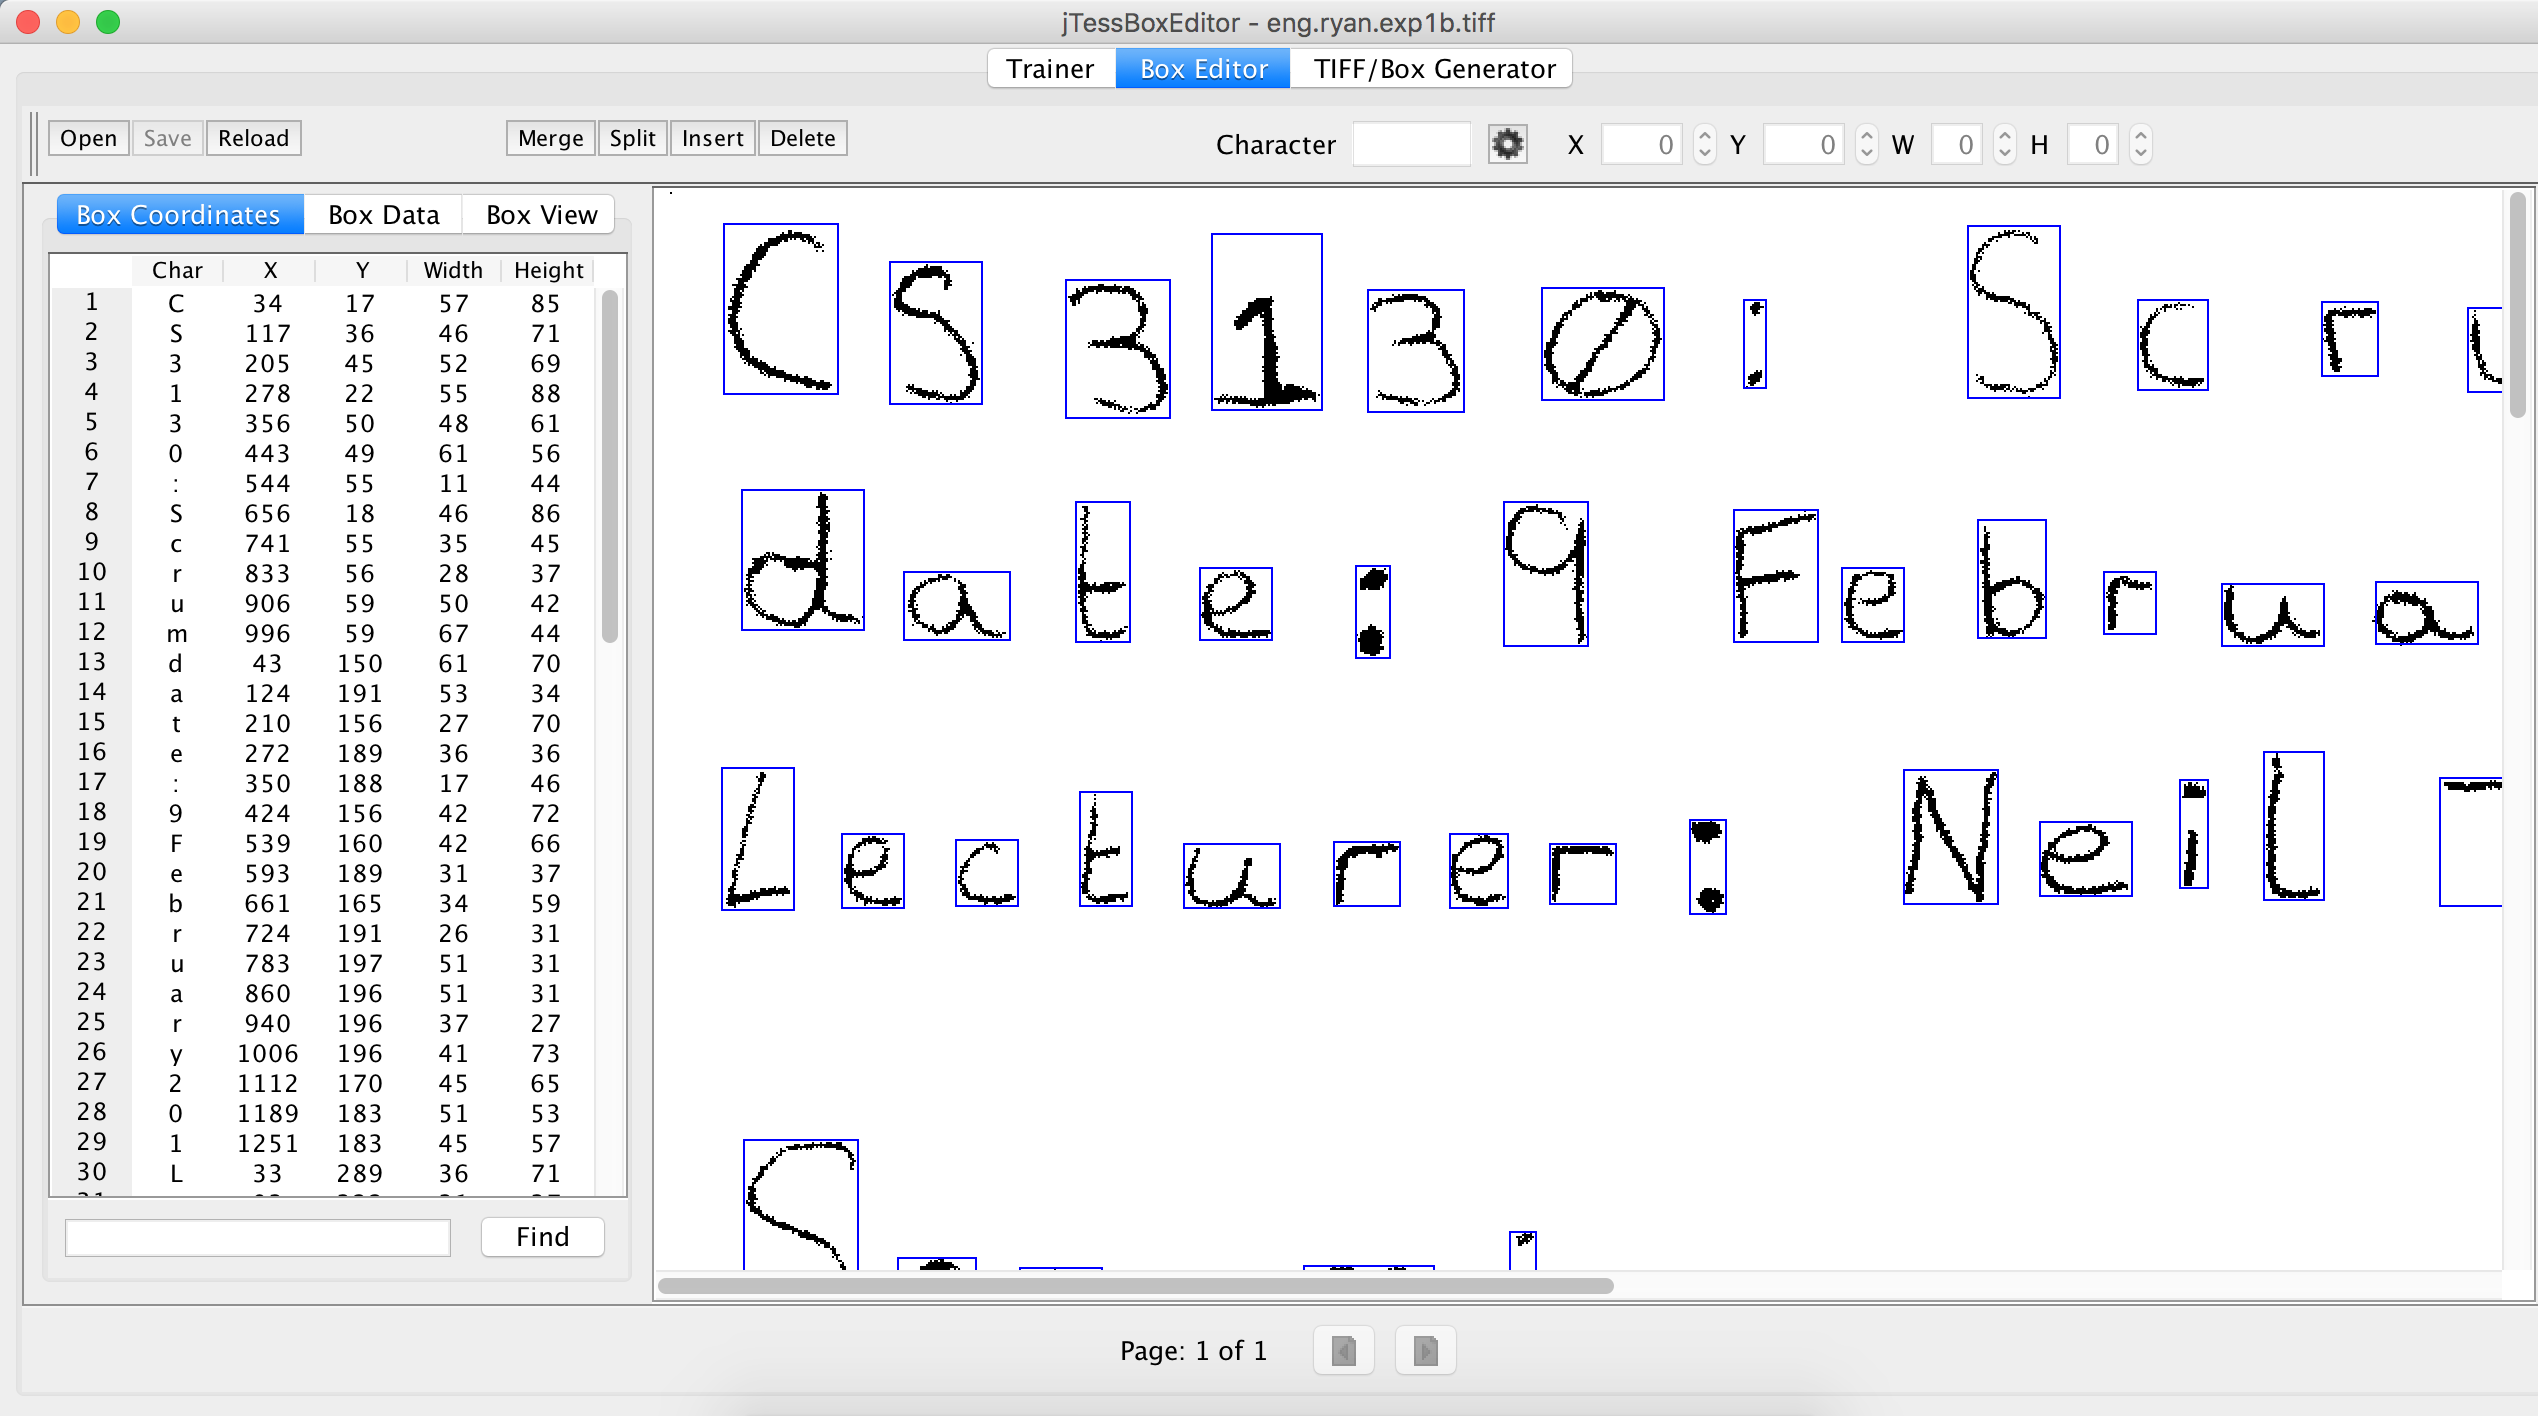
\includegraphics[width=\textwidth]{images/box_editor}
  \caption{A example of the jTessBoxEditor being used identify characters in the tiff box file.}
  \label{fig:box_editor}
\end{figure}

{{\ttfamily \hyphenchar\the\font=`\-}%
Once the characters had been manually changed, the box file was passed through Tesseract's training process. \texttt{tesseract <file> -l eng.ryan.exp2a box.train} would train the engine on the image's box file, for the language \texttt{eng.ryan.exp2a}. Often there were issues with being unable to identify tagged characters; these box file lines were deleted.

{{\ttfamily \hyphenchar\the\font=`\-}%
Following this process, Tesseract required an additional file ( \texttt{unicharset}) to be able to extract all possible characters that is identified in the training examples.

{{\ttfamily \hyphenchar\the\font=`\-}%
Tesseract's GitHub repository states that clustering is an important process to extract ``prototypes''. The clustering commands aid in ensuring the shapes of the characters tagged and identified are known so they can be used as a reference again.

A frequent words file was created, from the \texttt{/usr/share/dict/words} directory, to help to identify common words. This would aid in improving the chances of detecting specific words. Common words could also be defined; ``by'' and ``date'' are examples of words in this file.

{{\ttfamily \hyphenchar\the\font=`\-}%
Finally, the \texttt{combine\_data} command was used to combine all the data together and output a trained data file in the form of \texttt{eng.ryan.exp2a.trainedddata}. This was then copied to the shared Tesseract data directory enabling new training data to use this language.

{{\ttfamily \hyphenchar\the\font=`\-}%
Reinforcement of the characters identified was needed, so further training examples were created. This was called ``bootstrapping''. Therefore when training on another example, if the language was set to \texttt{eng.ryan.exp2a} it would reinforce that specific language with new data.

Throughout the sprints issues were identified whilst training the data. Characters would often not be identified correctly on the image, with specific issues with the letter ``g''  identified as a 3. When a blob could not be identified at all, Tesseract would label it $``\thicksim''$; these were ultimately removed when it was discovered that it would fail to identify them if edited. The training was conducted on twelve training examples, a selection can be found in Appendix \ref{tesseract:training}.

\section{Web application}
The web application was the main part of the development and specific sections proved to be more complex than anticipated.

\subsection{OAuth}\label{app:oauth}
The Google OAuth integration was more complex than first considered. Google suggested to use the Google client library \cite{citeulike:14024993} for all OAuth requests, to avoid security issues when making requests. Therefore, this library was utilised throughout the project.

The Google API client would, on occasion, raise peculiar errors. Whilst making a query to the calendar API it would raise the error, ``rootURL'', when using the build API call. This was mystifying as it was previously working. An issue was raised on the library's GitHub repository \cite{citeulike:14021433}. To confuse matters more, when querying the Google people plus API, it would work perfectly fine - however the Google calendar API would raise an exception. It eventually stopped throwing an exception, but the reason is unknown.

OAuth2 was implemented in the application so when the user clicks ``authorise with Google'' it will initialise the process for OAuth.
Once the user accepts the use of selected services a secure JSON credential file was returned containing specific tokens used when querying; these are appended to the user's session.

The credentials contain an expiration time, as shown in Appendix \ref{oauth:response}. When making a request this expiration time was checked, and if it was exceeded, then an error would be raised when querying the API's and displayed to the user. To overcome this, additional checks were made to ensure the credentials in the session were still valid. If they were not then it would redirect the user to the log-out route, clearing the session and asking the user to re-authenticate.

\subsection{Reoccuring events}
Reoccurring events within the Google Calendar integration, poised a lot of issues. It was identified in the pre-beta testing that if the user has a reoccurring event then it would not append the URL of the note to the event.

When a query was made for a list of events if there were reoccurring events then it would group the events by the first instance of these events. This proved to be problematic as it would display to the user that the note was taken on the 12th March, for example, but there were events from February being shown.

To account for this, the structure of the response was analysed and it was identified that grouped events had a \texttt{reoccurrenceID} key. After finding that the calendar API can fetch reoccurring items, a query was made using this ID key - filtering by the start and end date from the initial query. A check was included to ensure that when displaying to the user the event did not contain the \texttt{reoccurrenceID} key ensuring the singular events were displayed to the user.

Editing a reoccurring event produced further unexpected behaviour: when the event had been successfully modified and the note URL had been appended, it returned both the grouped event and the modified edited event in the initial query. Google must classify that changed reoccurring events as new instances. Instead of displaying more duplicated events to the user, a check for the \texttt{recurringEventId} key, which was present in the modified event, was conducted; if it was present the event was omitted.

Another issue identified were all-day events. All-day events do not have a datetime key in their start response field, returned from the Google Calendar API. This would cause the application to raise an exception and prevent the user from adding a note. A check was made to make sure that the datetime key was present.

\subsection{Tesseract confidence}
Displaying the Tesseract data went through a series of iterations over the latter sprints.

At a basic level integrating Tesseract into the web application was fairly simple and was implemented around sprint eight. The binarisation script, see Section \ref{imp:image_proces}, was incorporated to the application. This was added to the file upload route, as the user's image needs to be binarised when it is uploaded. A Tesseract wrapper could have been implemented but due to time constraints a 3rd party library, tesserocr \cite{citeulike:14021437}, was used.

\begin{figure}[H]
  \centering
  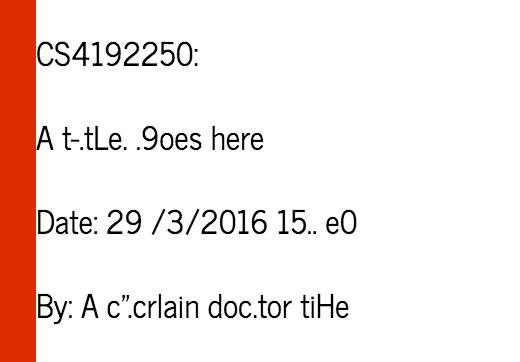
\includegraphics[scale=0.7]{images/tesseract_first}
  \label{fig:tesseract_output}
  \caption{Tesseract being integrated into the application at a very basic level}
\end{figure}

Tesserocr is a Python implementation of Tesseract's  C++ API. Tesserocr uses textlines to extract the text from the uploaded image. The first three lines were then iterated over, identifying the box for the lines so that text could be extracted. Each of these lines mapped the words identified and the confidence score for each word on a scale of 0 - 100 (0 being uncertain and 100 being certain).

The module code, lecturer, location and date were extracted via list-comprehensions, matching metadata structure defined in Section \ref{design:tesseract}. Modifications to the confidence scores were attempted in the controller to replace with a class name for the colours - so that the view file could render the content easily. Problems were encountered when the API returned tuples, an immutable type, so modification was not as eloquent as originally envisaged, therefore numbers remained.

Conditional checks were made in the view files on the confidence score; 75 would be green text, less than 74 and greater than 70 would be orange text and below 65 would be red text. Figure \ref{fig:tesseract_colour} shows the resulting output from the conditional checks. There are anomalies, with ``Date'' for example, it is orange but in-fact it is extracted perfectly.
\begin{figure}[H]
  \centering
  \begin{subfigure}[h]{0.35\textwidth}
    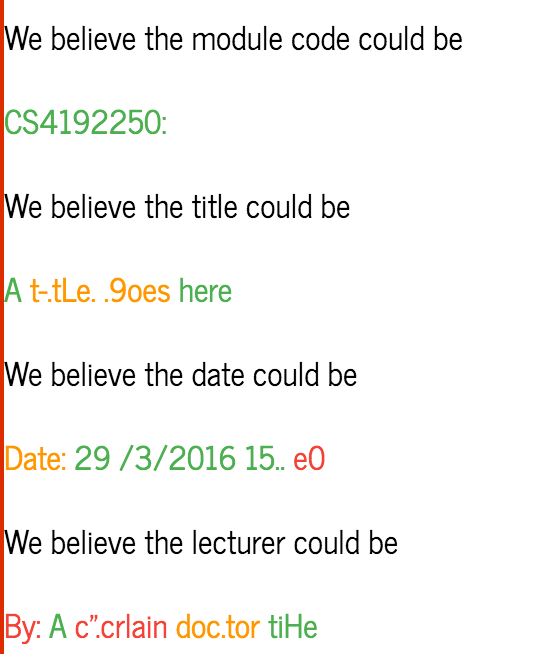
\includegraphics[scale=0.35]{images/tesseract_colour}
    \caption{}
    \label{fig:first_tesseract}
  \end{subfigure}
  \hspace{1em}
  \begin{subfigure}[h]{0.35\textwidth}
    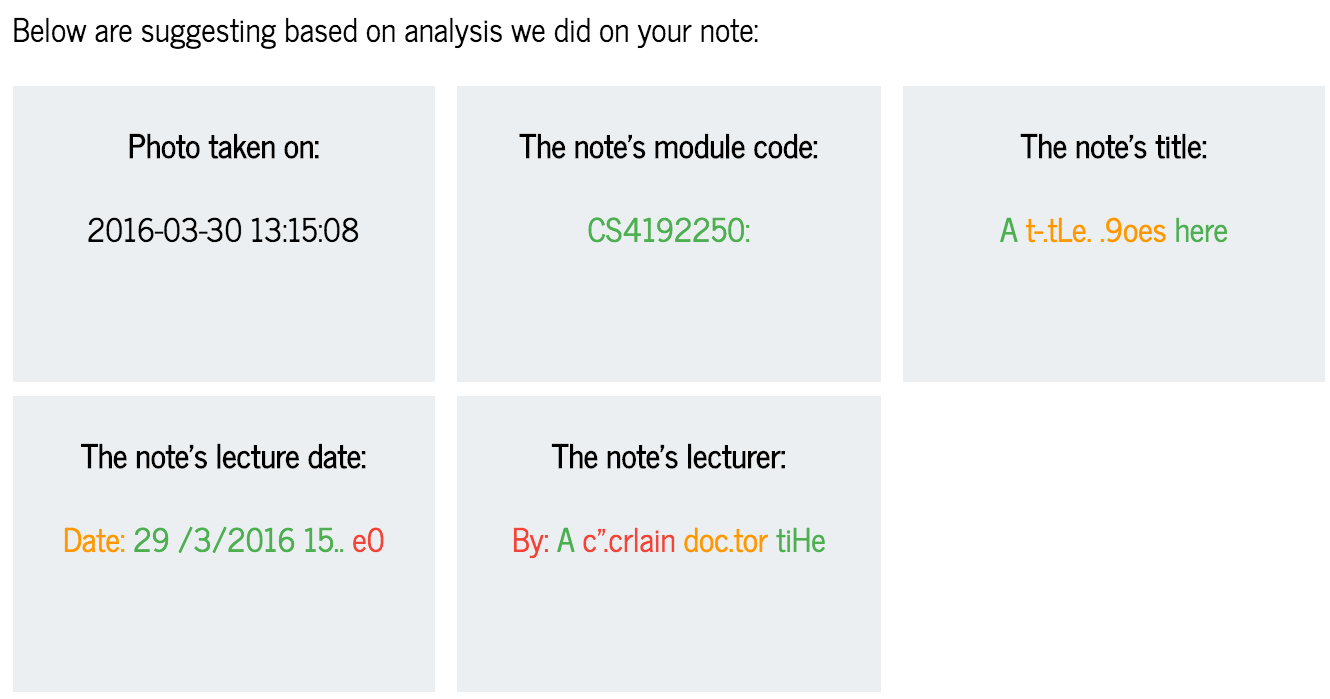
\includegraphics[scale=0.3]{images/styled-tesseract-data}
    \caption{}
    \label{fig:second_tesseract}
  \end{subfigure}
  \caption{Coloured representation of the confidence of the words from the handwriting: a) shows the initial steps with the image. b) shows the resulting output after styling of the web application}
  \label{fig:tesseract_colour}

\end{figure}

\subsection{Parsing EXIF data}
EXIF data parsing would be an important section of the application. EXIF data is essentially metadata about an image \cite{citeulike:14024991}. When a user uploads a note, it analyses the image for the EXIF metadata; it  uses the date of the image taken to query Google Calendar for additional events.

Throughout the sprints the EXIF data parsing was extended to allow for a greater variation in images uploaded. Python's image library \cite{citeulike:14024992} was used to parse the data. Further additional checks were made to ensure that the images were either JPEG or TIFF as they only contain the metadata.

During user-testing issues arose where a participant could not upload their note successfully. The image was formatted a JPEG but the mobile phone photo did not contain the ``dateTime'' EXIF key. Checks were implemented to ensure that this key existed.

\subsection{Displaying calendar events}
Over several user stories displaying different events around the application were created. The first instance of displaying the events were incorporated into the homepage, displaying the last seven days worth of events from the user, shown in Figure \ref{fig:seven_days}. This was simple to implement but provided a strong foothold into the interactions with the Google Calendar API; this stretched from the application to the testing infrastructure.

\begin{figure}[H]
  \centering
  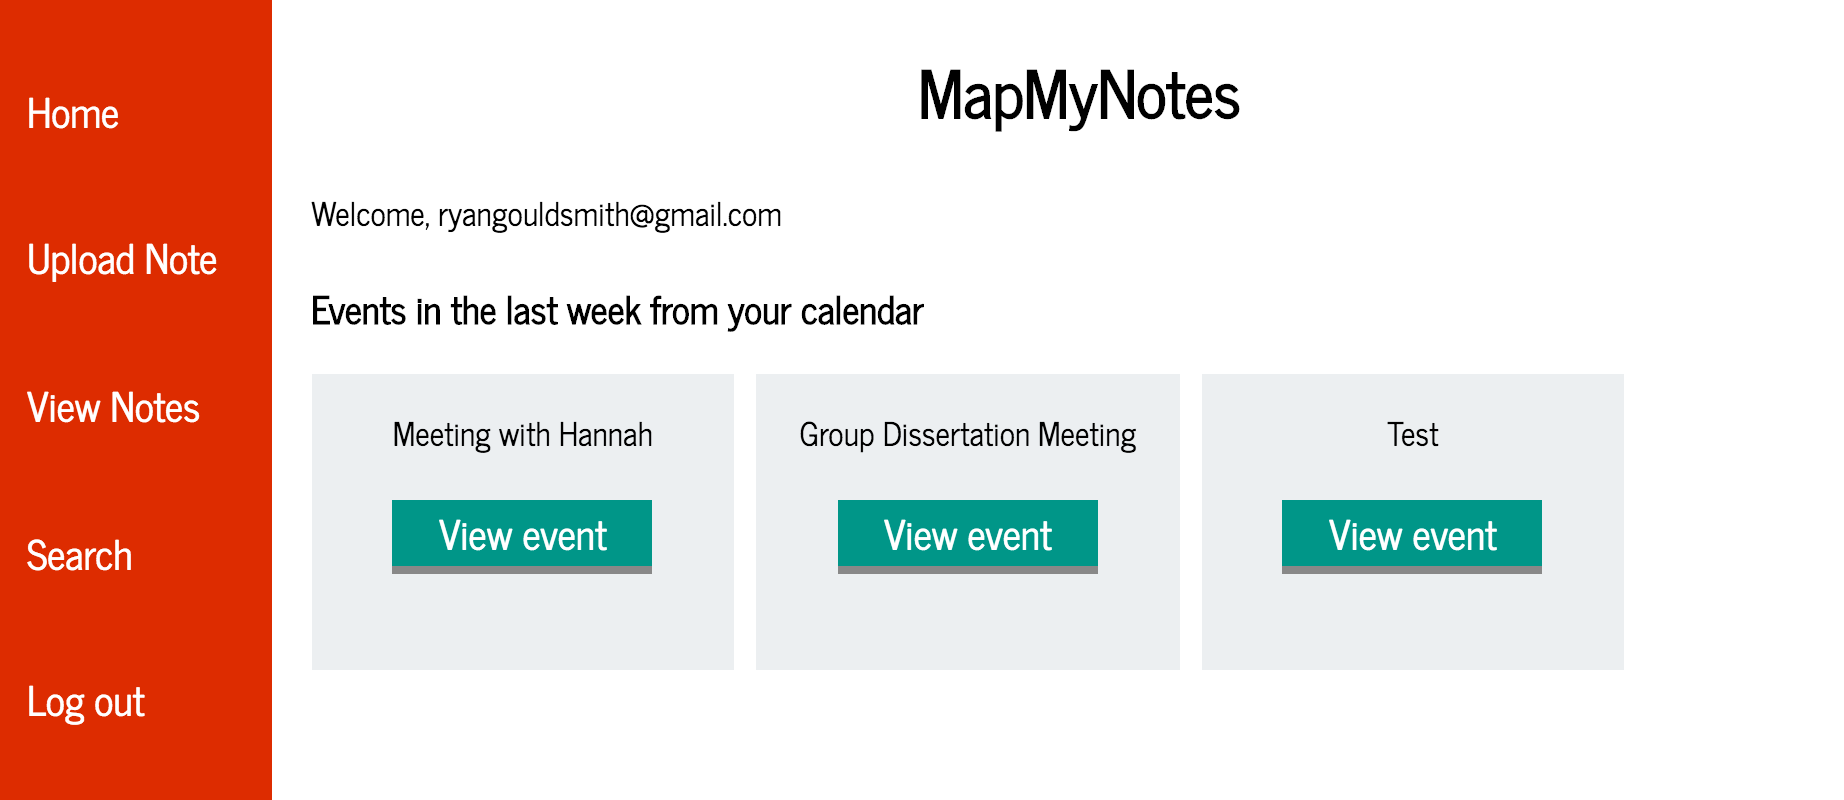
\includegraphics[scale=0.5]{images/event_seven_day}
  \caption{An example of displaying the events from the last week from the user's calendar}
  \label{fig:seven_days}
\end{figure}

One issue which arose was the change in timezones to British summer time during the project. If there was an event starting at 14:00, and the user queried for events at 14:00, then it would not return any results from the Google Calendar. Upon closer inspection if the query was for 13:00 then it would return the correct event. This issue rendered the application to a halt whilst this could be fixed: eventually, the timezone was appended to the user's input and querying with the timezone included returned the correct event from Google.

\subsection{Editing calendar events}
The user story for adding a note was implemented and as part of the tasks for this story, the note URL must be saved in the calendar event. When the user enters the date into the form, a query would be made to the Google Calendar API to return all associated events from that given day. Checks were then performed to ensure that the module code and the summary of the event matched.

This poised the problem of being able to add the note's URL to the correct event; if there was more than one event with the same module code that day then there could be confusion as to which event to add to.
Over the next iteration of development, the calendar events were additionally validated against the start date from the event and the user's input.

One issue which arose when adding the note's URL to the description field of the calendar was that it would replace the original content inside the description. This is a major concern for the users of the application as it would overwrite any data. Another issue it created was that multiple notes could not be attached to a given event. This was changed so that it would append to the description field, rather than overwriting it.

The algorithm for adding to a calendar is stated below.
\begin{algorithm}
  \caption{Adding a note URL to the calendar}
  \label{algorithm:threshold1}
  \begin{algorithmic}[1]
      \State Create a calendar service object
      \State Prepare URL from saved note
      \State Build the HTTP request
      \State Find an event for that day from the start time as given
      \State Parse the events
      \State Check to see if the summary contains module code AND the start date time matches
      \If{contains module code}
        \State check the response to see if description includes URL
        \State Save URL to the notes attribute in the database
      \EndIf
  \end{algorithmic}
\end{algorithm}

\begin{figure}[H]
  \centering
  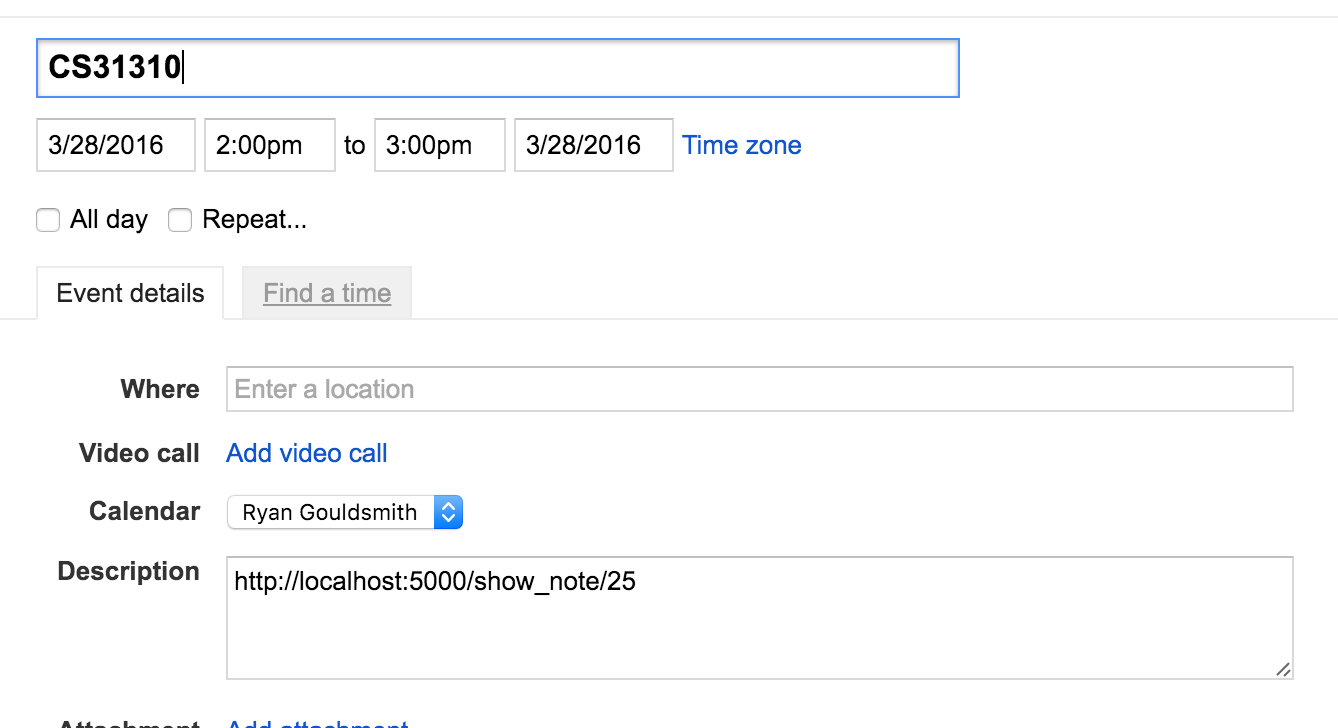
\includegraphics[scale=0.4]{images/saved_to_calendar}
  \caption{Saving a note correctly to a calendar event item}
  \label{fig:saved_to_calendar}
\end{figure}

Figure \ref{fig:saved_to_calendar} shows the output from saving a note to a specific date and appending the note's URL to the description field.

\subsubsection{Editing a note}
The user story ``editing a note'' was established midway through the project, an example task included when editing a note's start date it should be reflected in the user's calendar. If the user changes their date then it should remove the URL from the old calendar item and append to a new one, if the event exists. This proved to be a complicated implementation.

When a user edits a note it would query the API to return the event for the given note, based on the time start which was persisted for the note's relation. This event was then modified by replacing the description field with an empty string, replacing all the content. This caused issues regarding the data stored by the user being deleted arbitrarily. As a result a find and replace was used on the description field to remove any strings which matched the URL.

It is worth acknowledging at this point in the development considerable aspects of the codebase was refactored. There was duplicated functionality spread across multiple blueprints, making the codebase obfuscated. As a result the design decision for the \texttt{GoogleServicesHelper} emerged to abstract the duplication.

\subsubsection{Logging in and out}
Enabling the system to have users was an emerging user story midway through the project. As the log in would be deferred to Google, then the user would need to connect to the service. When the log in process has been completed a user's email address is extracted from the Google Plus API response and created in the database.

Using the application it was noticed that multiple user's were being created for a single email address. To reduce this problem a helper function was implemented which would find a user from their email address, if the user could not be found then they were added to the relation.

The user's ID is then appended to the session. Every page on the application verifies that this key exists. Once a user had finished using the application, the log-out route would destroy the user's session.

Delegating the responsibility to Google was a good design decision; the security which Google have would have been better than what could be implemented by the author. Furthermore, ethically, the only person information the system uses from a user is their email address.

\section{Travis}
Although not strictly a coding implementation, Travis formed a core part of the application and issues were found whilst using Travis.

Firstly, at the start of the process extensive time was invested into trying to  auto-deploy from Travis. Whilst giving detailed instructions on how to deploy to 3rd party systems the documentation for deployment to a virtual private server was sparse. Over several sprints the auto-deploy pipeline was desired but due to the lack of documentation there was no auto-deployment from Travis to a server.

When integrating Tesseract with the application, it became apparent of another issue with Travis: Tesseract and OpenCV had to be both built from source. TesserOCR uses Tesseract 3.04, and at the time of writing, Ubuntu's latest package is 3.02; this is the same for OpenCV 3.0.0. As a result, the build time for Travis was increased exponentially. The current build time was around thirty minutes; caching was investigated but no suitable solution was identified.
